\chapter{Basic Topology}\label{chap:basic-topology}
\begin{summary}
\item Metric space, subspace. Open ball, closed ball, boundedness. Open set, closed set. Interior, closure, boundary. Limit point.  
\item Compactness. Cantor intersection theorem, Heine--Borel theorem, Bolzano--Weierstrass theorem. Sequential compactness.
\item Perfect sets. Cantor set.
\item Connectedness.
\end{summary}

\begin{table}[H]
\centering
\begin{tabular}{cc}
\textbf{Term} & \textbf{Notation}\\
metric space & $X$, $Y$\\
metric & $d(p,q)$\\
general set & $E$\\
point in a set & $p$, $q$, $r$\\
open ball & $B_r(p)$\\
closed ball & $\overline{B}_r(p)$\\
punctured ball & $B_r^\prime(p)$\\
neighbourhood & $N$\\
interior & $E^\circ$\\
closure & $\overline{E}$\\
boundary & $\partial E$\\
induced set & $E^\prime$\\
compact set & $K$\\
open cover & $\mathcal{U}$\\
$n$-cell & $I$\\
Cantor set & $C$
\end{tabular}
\caption{Notation for topological structures in \cref{chap:basic-topology}}
\end{table}
\pagebreak

\section{Metric Spaces}
\subsection{Definitions and Examples}
\begin{definition}[Normed space]
Let $X$ be a vector space. A \emph{norm} is a function $\norm{\cdot}:X\to[0,\infty)$ if, for all $x,y\in X$ and constants $\alpha$,
\begin{enumerate}[label=(\roman*)]
\item $\norm{x}\ge0$, where equality holds if and only if $x=0$;\hfill(positive definiteness)
\item $\norm{\alpha x}=|\alpha|\norm{x}$;\hfill(homogeneity)
\item $\norm{x+y}\le\norm{x}+\norm{y}$.\hfill(triangle inequality)
\end{enumerate}
A \vocab{normed space}\index{normed space} $\brac{V,\norm{\cdot}}$ is a vector space $V$ together with a norm $\norm{\cdot}$.
\end{definition}

\begin{definition}[Metric space]
Let $X$ be a set. A \emph{metric} is a function $d:X\times X\to[0,\infty)$ if, for all $x,y,z\in X$,
\begin{enumerate}[label=(\roman*)]
\item $d(x,y)\ge0$, where equality holds if and only if $x=y$;\hfill(positive definiteness)
\item $d(x,y)=d(y,x)$;\hfill(symmetry)
\item $d(x,y)\le d(x,z)+d(z,y)$.\hfill(triangle inequality)
\end{enumerate}
A \vocab{metric space}\index{metric space} $(X,d)$ is a set $X$ together with a metric $d$.
\end{definition}

For the rest of the chapter, $X$ is taken to be a metric space, unless specified otherwise.

\begin{lemma}[Norm induces metric]
Let $X$ be a normed space. Then $X$ is a metric space, with the metric $d(x,y)=\norm{x-y}$ for every $x,y\in X$.
\end{lemma}

\begin{proof}
Trivial; check the conditions for a metric.
\end{proof}

\begin{example}[Metrics on $\RR^n$]
Each of the following functions define metrics on $\RR^n$.
\begin{align*}
d_1(x,y)&=\sum_{i=1}^{n}|x_i-y_i|;\\
d_2(x,y)&=\sqrt{\sum_{i=1}^{n}(x_i-y_i)}\\
d_\infty(x,y)&=\max_{i\in\{1,2,\dots,n\}}|x_i-y_i|.
\end{align*}
These are called the $\ell^1$-, $\ell^2$- (or Euclidean) and $\ell^\infty$-distances respectively.

The proof that each of $d_1$, $d_2$, $d_\infty$ is a metric is mostly very routine, with the exception of proving that $d_2$, the Euclidean distance, satisfies the triangle inequality. To establish this, recall that the Euclidean norm $\norm{x}_2$ of a vector $x=(x_1,\dots,x_n)\in\RR^n$ is
\[\norm{x}_2\colonequals\brac{\sum_{i=1}^n{x_i}^2}^\frac{1}{2}=\langle x,x\rangle^\frac{1}{2},\]
where the inner product is given by
\[\langle x,y\rangle\colonequals\sum_{i=1}^{n}x_i y_i.\]
Then $d_2(x,y)=\norm{x-y}_2$, and so the triangle inequality is the statement that
\[\norm{w-y}_2\le\norm{w-x}_2+\norm{x-y}_2.\]
This follows immediately by taking $u=w-x$ and $v=x-y$ in the following lemma.

\begin{lemma*}
If $u,v\in\RR^n$ then $\norm{u+v}_2\le\norm{u}_2+\norm{v}_2$.
\end{lemma*}

\begin{proof}
Since $\norm{u}_2\ge0$ for all $u\in\RR^n$, squaring both sides of the desired inequality gives
\[{\norm{u+v}_2}^2\le{\norm{u}_2}^2+2\norm{u}_2\norm{v}_2+{\norm{v}_2}^2.\]
But since
\[{\norm{u+v}_2}^2=\langle u+v,u+v\rangle={\norm{u}_2}^2+2\langle u,v\rangle+\norm{v}_2^2,\]
this inequality is immediate from the Cauchy--Schwarz inequality, that is to say the inequality
\[|\langle u,v\rangle|\le\norm{u}_2\norm{v}_2.\]
\end{proof}
\end{example}

\begin{comment}
\subsection{Norms}
\begin{definition}[Norms]
Let $V$ be any vector space (over the reals). A function $\norm{\cdot}:V\to[0,\infty)$ is called a \vocab{norm}\index{norm} if it satisfies the following properties:
\begin{enumerate}[label=(\roman*)]
\item $\norm{x}=0$ if and only if $x=0$;
\item $\norm{\lambda x}=|\lambda|\norm{x}$ for all $\lambda\in\RR$, $x\in V$;
\item $\norm{x+y}\le\norm{x}+\norm{y}$ for all $x,y\in V$.
\end{enumerate}
\end{definition}

Given a norm, it is very easy to check that $d(x,y)\colonequals\norm{x-y}$ defines a metric on $V$. Indeed, we have already seen that when $V=\RR^n$, $\norm{\cdot}_2$ is a norm (and so the name ``Euclidean norm'' is appropriate) and we defined $d_2(x,y)=\norm{x-y}_2$. The other metrics on $\RR^n$ also come from norms: $d_1$ comes from the $\ell^1$-norm
\[\norm{x}_1\colonequals\sum_{i=1}^n|x_i|,\]
whilst $d_\infty$ comes from the $\ell^\infty$-norm
\[\norm{x}_\infty\colonequals\max_{i=1,\dots,n}|x_i|.\]
More generally, the family of $\ell^p$-norms are given by
\[\norm{x}_p\colonequals\brac{\sum_{i=1}^n|x_i|^p}^\frac{1}{p}.\]

The principle of turning norms into metrics is important enough that we state it as a lemma in its own right.

\begin{lemma}
Let $V$ be a vector space over $\RR$, let $\norm{\cdot}$ be a norm on $V$. Define $d:V\times V\to[0,\infty)$ by $d(x,y)\colonequals\norm{x-y}$. Then $(V,d)$ is a metric space.
\end{lemma}

\begin{proof}
Simply verify the three axioms for a metric space, which directly correspond to the three axioms for a norm.
\end{proof}

\begin{remark}
The converse is very far from true. For instance, the discrete metric does not arise from a norm. All metrics arising from a norm have the \emph{translation invariance property} $d(x+z,y+z)=d(x,y)$, as well as the \emph{scalar invariance} $d(\lambda x,\lambda y)=|\lambda|d(x,y)$, neither of which are properties of arbitrary metrics.

Conversely one can show that a metric with these two additional properties does come from a norm, an exercise we leave to the reader. [Hint: the norm must arise as $\norm{v}=d(v,0)$.]
\end{remark}

We call a vector space endowed with a norm $\norm{\cdot}$ a \vocab{normed space}. Whenever we talk about normed spaces it is understood that we are also thinking of them as metric spaces, with the metric being defined by $d(v,w)=\norm{v-w}$.

Note that we do not assume that the underlying vector space $V$ is finite dimensional. Here are some examples which are not finite-dimensional (whilst we do not prove that they are not finite-dimensional here, it is not hard to do so and we suggest this as an exercise).

\begin{example}[$\ell^p$ spaces]
Let
\begin{align*}
\ell_1&=\crbrac{(x_n)_{n=1}^\infty\:\bigg|\:\sum_{n\ge1}|x_n|<\infty},\\
\ell_2&=\crbrac{(x_n)_{n=1}^\infty\:\bigg|\:\sum_{n\ge1}x_n^2<\infty},\\
\ell_\infty=&\crbrac{(x_n)_{n=1}^\infty\:\bigg|\:\sup_{n\in\NN}|x_n|<\infty}.
\end{align*}
The sets $\ell_1$, $\ell_2$, $\ell_\infty$ are all real vector spaces, and moreover
\begin{align*}
\norm{(x_n)}_1&=\sum_{n\ge1}|x_n|,\\
\norm{(x_n)}_2&=\brac{\sum_{n\ge1}x_n^2}^\frac{1}{2},\\
\norm{(x_n)}_\infty&=\sup_{n\in\NN}|x_n|
\end{align*}
define norms on $\ell_1$, $\ell_2$ and $\ell_\infty$ respectively.

Note that $\ell_2$ is in fact an inner product space where
\[\langle(x_n),(y_n)\rangle=\sum_{n\ge1}x_ny_n,\]
(the fact that the right-hand side converges if $(x_n)$ and $(y_n)$ are in $\ell_2$ follows from the Cauchy--Schwarz inequality). The space $\ell^2$ is known as \vocab{Hilbert space}.
\end{example}
\end{comment}

A metric space $(X,d)$ naturally induces a metric on any of its subsets.

\begin{definition}[Subspace]
Suppose $(X,d)$ is a metric space, $Y\subset X$. Then the restriction of $d$ to $Y\times Y$ gives $Y$ a metric
\[d_Y=d|_{Y\times Y},\]
so that $(Y,d_Y)$ is a metric space. We call $Y$ equipped with this metric a \vocab{subspace}.
\end{definition}
\pagebreak

\subsection{Balls and Boundedness}
\begin{definition}[Balls]\index{balls} \
\begin{enumerate}[label=(\roman*)]
\item The \vocab{open ball}\index{balls!open ball} centred at $x\in X$ with radius $r>0$ is the set
\[B_r(x)\colonequals\{y\in X\mid d(y,x)<r\}.\]
\item The \vocab{closed ball}\index{balls!closed ball} centred at $x$ with radius $r$ is
\[\overline{B}_r(x)\colonequals\{y\in X\mid d(y,x)\le r\}.\]
\item The \vocab{punctured ball}\index{balls!punctured ball} is the open ball excluding its centre:
\[B_r^\prime(x)\colonequals\{y\in X\mid 0<d(y,x)<r\}.\]
\end{enumerate}
\end{definition}

\begin{figure}[H]
\centering
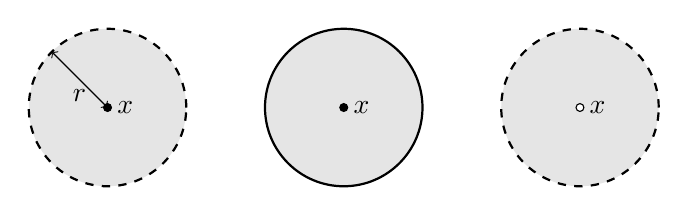
\begin{tikzpicture}
\filldraw[color=black, dashed, fill=gray!20, thick](0,0) circle (1.0cm);
\draw[fill=black] (0,0) circle[radius=0.05cm] node [anchor=west] {$x$};
\draw[<->] (0,0) -- (-0.71,0.71) node [midway, below] {$r$};

\filldraw[color=black, fill=gray!20, thick](3,0) circle (1.0cm);
\draw[fill=black] (3,0) circle[radius=0.05cm] node [anchor=west] {$x$};

\filldraw[color=black, dashed, fill=gray!20, thick](6,0) circle (1.0cm);
\draw[fill=white] (6,0) circle[radius=0.05cm] node [anchor=west] {$x$};
\end{tikzpicture}
\caption{Open ball, closed ball, punctured ball}
\end{figure}

\begin{example}
Considering $\RR^3$ with the Euclidean metric, $B_1(0)$ really is what we understand geometrically as a ball (minus its boundary, the unit sphere), whilst $\overline{B}_1(0)$ contains the unit sphere and everything inside it.
\end{example}

\begin{remark}
We caution that this intuitive picture of the closed ball being the open ball ``together with its boundary'' is totally misleading in general. For instance, in the discrete metric on a set $X$, the open ball $B_1(x)$ contains only the point $x$, whereas the closed ball $\overline{B}_1(x)$ is the whole of $X$.
\end{remark}

\begin{definition}[Bounded]
We say $E\subset X$ is \vocab{bounded}\index{boundedness} if $E$ is contained in some open ball; that is, there exists $M\in\RR$ and $x\in X$ such that $E\subset B_M(x)$.
\end{definition}

\begin{figure}[H]
\centering
\begin{tikzpicture}
\filldraw[color=black, dashed, fill=gray!20, thick](0.9,1.5) circle (2.6cm);
\draw[fill=black] (0.9,1.5) circle[radius=0.05cm] node [anchor=west] {$x$};
%% Blob
\path[draw,use Hobby shortcut,closed=true]
(0,0) .. (.5,1) .. (1.5,3) .. (.3,4) .. (-1,2) .. (-1,.5);
\end{tikzpicture}
\caption{Bounded set}
\end{figure}

\begin{proposition}
Let $E\subset X$. Then the following are equivalent:
\begin{enumerate}[label=(\roman*)]
\item $E$ is bounded;
\item $E$ is contained in some closed ball;
\item The set $\{d(x,y)\mid x,y\in E\}$ is a bounded subset of $\RR$.
\end{enumerate}
\end{proposition}

\begin{proof} \

\fbox{(i)$\implies$(ii)} This is obvious.

\fbox{(ii)$\implies$(iii)} This follows immediately from the triangle inequality.

\fbox{(iii)$\implies$(i)} Suppose $E$ satisfies (iii), then there exists $r\in\RR$ such that $d(x,y)\le r$ for all $x,y\in E$. If $E=\emptyset$, then $E$ is certainly bounded. Otherwise, let $p\in E$ be an arbitrary point. Then $E\subset B_{r+1}(p)$.
\end{proof}

\begin{comment}
\begin{definition}[Diameter]
Let non-empty $E\subset X$. Then the \vocab{diameter} of $E$ is
\[\diam E\colonequals\sup_{p,q\in E}d(p,q).\]
\end{definition}

\begin{example}
Find the diameter of the open unit ball in $\RR^n$:
\[B=\{\vb{x}\in\RR^n\mid\norm{\vb{x}}<1\}. \]
\begin{proof}
Note that for all $\vb{x},\vb{y}\in\RR^n$,
\[d(\vb{x},\vb{y})=\norm{\vb{x}-\vb{y}}\le\norm{\vb{x}}+\norm{-\vb{y}}=\norm{\vb{x}}+\norm{\vb{y}}<1+1=2. \]
On the other hand, for any $\epsilon>0$, we pick
\[\vb{x}=\brac{1-\frac{\epsilon}{4},0,\dots,0},\quad\vb{y}=\brac{-\brac{1-\frac{\epsilon}{4}},0,\dots,0}. \]
Then $d(\vb{x},\vb{y})=2-\dfrac{\epsilon}{2}>2-\epsilon$. Since $\epsilon$ is arbitrary, we have that $\diam B=2$.
\end{proof}
\end{example}

\begin{proposition}
$E\subset\RR^n$ is bounded if and only if $\diam E<+\infty$.
\end{proposition}

\begin{proof} \

\forward If $E$ is bounded, then there exists $M>0$ such that $\norm{x}\le M$ for all $x \in E$.

Thus for any $x,y \in E$,
\[ d(x,y)=\norm{x-y}\le\norm{x}+\norm{y}\le2M. \]
Thus $\diam E = \sup d(x,y) \le 2M<+\infty$.

\backward Suppose that $\diam E=r$. Pick a random point $x\in E$, suppose that $\norm{x}=R$.

Then for any other $y \in E$,
\[ \norm{y}=\norm{x+(y-x)}\le\norm{x}+\norm{y-x}\le R+r. \]
Thus, by picking $M=R+r$, we obtain $\norm{y}\le M$ for all $y \in E$, and we are done.
\end{proof}

\begin{remark}
Basically we used $x$ to confine $E$ within a ball, which is then confined within an even bigger ball centered at the origin.
\end{remark}
\end{comment}
\pagebreak

\subsection{Open and Closed Sets}
We say $N\subset X$ is a \vocab{neighbourhood}\index{neighbourhood} of $x\in X$ if there exists $\epsilon>0$ such that $B_\epsilon(x)\subset N$.

\begin{definition}[Open set]
We say $E\subset X$ is \vocab{open}\index{open set} (in $X$) if it is a neighbourhood of all its elements; that is, for all $x\in E$, there exists $\epsilon>0$ such that $B_\epsilon(x)\subset E$.
\end{definition}

\begin{figure}[H]
\centering
\begin{tikzpicture}
%% Blob
\path[draw,use Hobby shortcut,closed=true]
(0,0) .. (.5,1) .. (1.5,3) .. (.3,4) .. (-1,2) .. (-1,.5);
\filldraw[color=black, dashed, fill=gray!20, thick](0,1.5) circle (0.6cm);
\draw[fill=black] (0,1.5) circle[radius=0.05cm] node [anchor=west] {$x$};
\end{tikzpicture}
\caption{Open set}
\end{figure}

\begin{lemma}
Any open ball is open.
\end{lemma}

\begin{figure}[H]
\centering
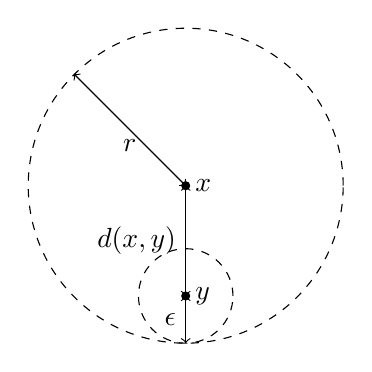
\begin{tikzpicture}
\draw[dashed] (0,0) circle[radius=2.0cm];
\draw[fill=black] (0,0) circle[radius=0.05cm] node [anchor=west] {$x$};
\draw[<->] (0,0) -- (-1.42,1.42) node [midway, below] {$r$};

\draw[dashed] (0,-1.40) circle[radius=0.6cm];
\draw[fill=black] (0,-1.40) circle[radius=0.05cm] node [anchor=west] {$y$};
\draw[<->] (0,0) -- (0,-1.40) node [midway, left] {$d(x,y)$};
\draw[<->] (0,-1.40) -- (0,-2) node [midway, left] {$\epsilon$};
\end{tikzpicture}
\end{figure}

\begin{proof}
Let $B_r(x)$ be an open ball. 

Let $y\in B_r(x)$. To show that $B_r(x)$ is open, we will show that $B_\epsilon(y)\subset B_r(x)$ for some $\epsilon>0$.

Take $\epsilon=r-d(x,y)$. 
Let $z\in B_\epsilon(y)$. By the triangle inequality,
\begin{align*}
d(x,z)&\le d(y,z)+d(x,y)\\
&<\epsilon+d(x,y)=r
\end{align*}
so $z\in B_r(x)$, which implies $B_\epsilon(y)\subset B_r(x)$.
\end{proof}

\begin{lemma}\label{lemma:open-set-properties} \
\begin{enumerate}[label=(\roman*)]
\item Both $\emptyset$ and $X$ are open.
\item For any indexing set $I$ and collection of open sets $\{E_i\mid i\in I\}$, $\bigcup_{i\in I}E_i$ is open.
\item For any \emph{finite} indexing set $I$ and collection of open sets $\{E_i\mid i\in I\}$, $\bigcap_{i\in I}E_i$ is open.
\end{enumerate}
\end{lemma}

\begin{proof} \
\begin{enumerate}[label=(\roman*)]
\item Obvious by definition.
\item If $x\in\bigcup_{i\in I}E_i$, then $x\in E_i$ for some $i\in I$. Since $E_i$ is open, there exists $\epsilon>0$ such that $B_\epsilon(x)\subset E_i$ and hence $ B_\epsilon(x)\in\bigcup_{i\in I}E_i$.
\item Suppose $I$ is finite and $x\in\bigcap_{i\in I}E_i$. For each $i\in I$, we have $x\in E_i$ and so there exists $\epsilon_i$ such that $B_{\epsilon_i}(x)\subset E_i$. Set $\epsilon=\min_{i\in I}\epsilon_i$, then $\epsilon>0$ (here it is, of course, crucial that $I$ be finite), and $B_\epsilon(x)\subset B_{\epsilon_i}(x)\subset E_i$ for all $i$. Therefore $ B_\epsilon(x)\subset\bigcap_{i\in I}E_i$.
\end{enumerate}
\end{proof}

\begin{remark}
While the indexing set $I$ in (ii) can be arbitrary, the indexing set in (iii) must be finite. For instance, $E_n=\brac{-\frac{1}{n},\frac{1}{n}}$ are open in $\RR$, but their intersection $\bigcap_{n=1}^\infty E_n=\{0\}$ is not open.
\end{remark}

Suppose $Y$ is a subspace of $X$. We say that $E$ is \emph{open relative} to $Y$ if for all $p\in E$, there exists $\epsilon>0$ such that $B_\epsilon(p)\cap Y\subset E$. (Note that $B_\epsilon(p)\cap Y$ is in the open ball in $Y$\footnote{notice that the definition of an open ball depends on the metric space!}, because the metric $d^\prime:Y\times Y\to R$ is the restriction to $Y\times Y$ of the metric $d:X\times X\to\RR$ on $X$.)

\begin{proposition}\label{prop:open-subspace-cap}
Suppose $Y$ is a subspace of $X$, $E\subset Y$. Then $E$ is open relative to $Y$ if and only if there exists an open subset $G$ of $X$ such that $E=Y\cap G$.
\end{proposition}

\begin{proof} \

\forward We prove by construction; that is, construct the required set $G$.

Suppose $E$ is open relative to $Y$. For each $p\in E$, by openness of $E$, there exists $r_p>0$ such that $B_{r_p}(p)\cap Y\subset E$.
Consider the union
\[\bigcup_{p\in E}\brac{B_{r_p}(p)\cap Y}\subset E.\]
Note that we can write
\[\bigcup_{p\in E}\brac{B_{r_p}(p)\cap Y}=\brac{\bigcup_{p\in E}B_{r_p}(p)}\cap Y\subset E.\]
Let
\[G=\bigcup_{p\in E}B_{r_p}(p),\]
then we have $G\cap Y\subset E$. 

Since $G$ is an intersection of open balls (which are open sets), by \ref{lemma:open-set-properties}, $G$ is an open subset of $X$.

Note for each $p\in E\subset Y$, we have $p\in Y$, and $p\in B_{r_p}(p)$ for some $r_p>0$, so $p\in\bigcup_{p\in E}B_{r_p}(p)=G$. Hence $p\in G\cap Y$. This shows $E\subset G\cap Y$.

Hence $E=G\cap Y$.

\backward Suppose $E=G\cap Y$ for some open subset $G$ of $X$. 

Let $p\in E$. Since $p\in G$, by the openness of $G$, there exists $r_p>0$ such that $B_{r_p}(p)\subset G$. Then $B_{r_p}(p)\cap Y\subset G\cap Y=E$. Thus by definition $E$ is open relative to $Y$.
\end{proof}

The complement of an open set is a \emph{closed} set.

\begin{definition}[Closed set]
We say $E\subset X$ is \vocab{closed}\index{closed set} if its complement $E^c=X\setminus E$ is open.
\end{definition}

\begin{lemma}
Any closed ball is closed.
\end{lemma}

\begin{proof}
To prove that $\overline{B}_r(p)$ is closed, we need to show that its complement
\[\overline{B}_r(p)^c=\{q\in X\mid d(p,q)>r\}\]
is open.

Let $s\in\overline{B}_r(p)^c$. Take $\epsilon>0$ such that $r+\epsilon<d(p,s)$; that is, $\epsilon<d(p,s)-r$.

Let $q\in B_\epsilon(s)$, then $d(q,s)<\epsilon$. Thus $d(q,s)<d(p,s)-r$, or $r<d(p,s)-d(q,s)$. Then by the triangle inequality,
\begin{align*}
d(p,q)&\ge d(p,s)-d(q,s)\\
&>r
\end{align*}
Hence $q\in\overline{B}_r(p)^c$, and so $B_\epsilon(s)\subset\overline{B}_r(p)^c$. Therefore $\overline{B}_r(p)^c$ is open, so $\overline{B}_r(p)$ is closed.
\end{proof}

\begin{lemma}\label{lemma:closed-set-properties} \
\begin{enumerate}[label=(\roman*)]
\item Both $\emptyset$ and $X$ are closed.
\item For any indexing set $I$ and collection of closed sets $\{F_i\mid i\in I\}$, $\bigcap_{i\in I}F_i$ is closed.
\item For any \emph{finite} indexing set $I$ and collection of closed sets $\{F_i\mid i\in I\}$, $\bigcup_{i\in I}F_i$ is closed.
\end{enumerate}
\end{lemma}

\begin{proof}
From \ref{lemma:open-set-properties}, simply take complements and apply de Morgan's laws.
\end{proof}

\begin{remark}
The indexing set in (iii) must be finite; for instane, the closed intervals $F_n=\sqbrac{-1+\frac{1}{n},1-\frac{1}{n}}$ are all closed in $\RR$, but their union $\bigcup_{n=1}^\infty F_n=(-1,1)$ is open.
\end{remark}
\pagebreak

\subsection{Interior, Closure, Boundary}
\begin{definition}
Suppose $E\subset X$.
\begin{enumerate}[label=(\roman*)]
\item The \vocab{interior}\index{interior} $E^\circ$ of the set $E$ is the union of all open subsets of $X$ contained in $E$; we call $p\in E^\circ$ an \vocab{interior point} of $E$. 

\item The \vocab{closure}\index{closure} $\overline{E}$ of the set $E$ is the intersection of all closed subsets of $X$ containing $E$.

We say $E$ is \vocab{dense}\index{dense} if $\overline{E}=X$. 

\item The \vocab{boundary}\index{boundary} of $E$ is $\partial E=\overline{E}\setminus E^\circ$; we call $p\in\partial E$ a \vocab{boundary point}\index{boundary point} of $E$.
\end{enumerate}
\end{definition}

In the figure below, the black outline represents the boundary; the grey area within represents the interior; the union represents the closure.
\begin{figure}[H]
\centering
\begin{tikzpicture}
%% Blob
\path[draw,use Hobby shortcut,closed=true, fill=gray!20]
(0,0) .. (.5,1) .. (1.5,3) .. (.3,4) .. (-1,2) .. (-1,.5);
\end{tikzpicture}
\caption{Interior, closure, boundary}
\end{figure}

\begin{example} \
\begin{itemize}
\item The interior of the closed interval $[a,b]$ is the open interval $(a,b)$.
\item $\QQ$ is dense in $\RR$.
\end{itemize}
\end{example}

\begin{remark}
$E$ and $E^\circ$ do not necessarily have the same closures; for example, take $E=\QQ$, then $\overline{E}=\RR$ and $\overline{E^\circ}=\emptyset$.

Likewise, $E$ and $\overline{E}$ do not necessarily have the same interiors; for example, take $E=(-1,0)\cup(0,1)\subset\RR$. Then $E^\circ=(-1,0)\cup(0,1)$ and $(\overline{E})^\circ=[-1,1]$.
\end{remark}

\begin{lemma}
Suppose $E\subset X$.
\begin{enumerate}[label=(\roman*)]
\item $E$ is open if and only if $E=E^\circ$.

(That is, $E$ is open if and only if every point of $E$ is an interior point.)

\item $E$ is closed if and only if $E=\overline{E}$.
\end{enumerate}
\end{lemma}

\begin{proof} \
\begin{enumerate}[label=(\roman*)]
\item \forward Suppose $E$ is open. By assumption, $E$ is an open subset of $X$ contained in $E$ (since $E\subset E$), so $E\subset E^\circ$. 

We now show the opposite containment. Let $x\in E^\circ$. Then $x$ is in some open subset of $X$ contained in $E$, so $x\in E$. Hence $E^\circ\subset E$. 

Therefore $E=E^\circ$.

\backward Since an arbitrary union of open sets is open, $E^\circ$ is open. Since $E=E^\circ$, we have that $E$ is open.

\item \forward Suppose $E$ is closed. Then $E\subset\overline{E}$. 

We now show the opposite containment. Let $x\in\overline{E}$. Then $x$ is in every closed subset of $X$ containing $E$, so $x\in E$. Hence $x\in E$.

Therefore $E=\overline{E}$.

\backward Since an arbitrary intersection of closed sets is closed, $\overline{E}$ is closed. Since $E=\overline{E}$, we have that $E$ is closed.
\end{enumerate}
\end{proof}

\begin{proposition}
Suppose $E\subset X$. Then $p\in\overline{E}$ if and only if every open ball centred at $p$ contains a point of $E$.
\end{proposition}

\begin{proof} \

\forward Let $p\in\overline{E}$. 

Suppose, for a contradiction, that there exists an open ball $B_\epsilon(p)$ that does not meet $E$. Then $B_\epsilon(p)^c$ is a closed set containing $E$. Therefore $B_\epsilon(p)^c$ contains $\overline{E}$, and hence it contains $p$, which is obviously nonsense.

\backward Suppose that every ball $B_\epsilon(p)$ meets $E$. 

Suppose, for a contradiction, that $p\notin\overline{E}$. 
Since $\overline{E}^c$ is open, there is a ball $B_\epsilon(p)$ contained in $\overline{E}^c$, and hence in $E^c$, contrary to assumption.
\end{proof}

\begin{remark}
A particular consequence of this is that $E\subset X$ is dense if and only if it meets every open set in $X$.
\end{remark}

\begin{lemma}[Properties of closure and interior]
Suppose $A,B\subset X$. Then
\begin{enumerate}[label=(\roman*)]
\item $\overline{A\cup B}=\overline{A}\cup\overline{B}$
\item $\overline{A\cap B}\subset\overline{A}\cap\overline{B}$
\item $(A\cup B)^\circ\supset A^\circ\cup B^\circ$
\item $(A\cap B)^\circ=A^\circ\cap B^\circ$
\item $(A^\circ)^c=\overline{A^c}$
\item $(\overline{A})^c=(A^c)^\circ$
\end{enumerate}
\end{lemma}
\pagebreak

\subsection{Limit Points}
\begin{definition} \
\begin{enumerate}[label=(\roman*)]
\item $p\in X$ (not necessarily in $E$) is an \vocab{adherent point} of $E$ (or is \emph{adherent} to $E$) if $B_\epsilon(p)\cap E\neq\emptyset$ for all $\epsilon>0$.
\item $p\in X$ is a \vocab{limit point}\index{limit point} of $E$ if, for all $\epsilon>0$, there exists $q\in E\setminus\{p\}$ such that $q\in B_\epsilon(p)$. (In other words, $p$ is a limit point of $E$ if and only if $p$ adheres to $E\setminus\{p\}$.)

The \vocab{induced set}\index{induced set} of $E$, denoted by $E^\prime$, is the set of all limit points of $E$ in $X$.

\item $p\in E$ is an \vocab{isolated point} of $E$ if $p$ is not an limit point of $E$ (that is, there exists $\epsilon>0$ such that $B_\epsilon(p)\cap E=\{p\}$).
\end{enumerate}
\end{definition}

\begin{figure}[H]
\centering
\begin{tikzpicture}
%% Blob
\path[draw,use Hobby shortcut,closed=true,dashed,fill=gray!20]
(0,0) .. (.5,1) .. (1.5,3) .. (.3,4) .. (-1,2) .. (-1,.5);
\draw[fill=black] (-1,2) circle[radius=0.05cm] node [anchor=east] {$a$};
\end{tikzpicture}
\caption{Adherent point, limit point, isolated point}
\end{figure}

\begin{example}[Adherent point] \
\begin{itemize}
\item If $p\in E$, then $p$ adheres to $E$ because every ball contains $p$.
\item If $E\subset\RR$ is bounded above, then $\sup E$ is adherent to $E$.
\end{itemize}
\end{example}

\begin{example}[Limit point] \
\begin{itemize}
\item The set $\crbrac{\frac{1}{n}\:\big|\:n\in\NN}$ has $0$ as a limit point.
\item The set of rational numbers has every real number as a limit point.
\item Every point of $[a,b]$ is a limit point of the set of numbers in $(a,b)$.
\item Consider $\RR^2$. The set of limit points of any open ball $B_r(p)$ is the closed ball $\overline{B}_r(p)$, which is also the closure of $B_r(p)$.
\item Consider $\QQ\subset\RR$. $\QQ^\prime=\overline{\QQ}=\RR$.
\end{itemize}
\end{example}

\begin{proposition}\label{prop:limit-point-inf-points}
If $p$ is a limit point of $E$, then every open ball of $p$ contains infinitely many points of $E$.
\end{proposition}

\begin{proof}
Suppose, for a contradiction, that there exists an open ball $B_r(p)$ which contains only a finite number of points of $E$ distinct from $p$; let
\[B_r(p)=\{q_1,\dots,q_n\},\]
where $p\neq q_i$ for $i=1,\dots,n$. 
Take
\[r=\min\{d(p,q_1),\dots,d(p,q_n)\},\]
then $B_r(p)$ contains no points of $E$ distinct from $p$, which is a contradiction.
\end{proof}

\begin{corollary}
A finite point set has no limit points.
\end{corollary}

\begin{remark}
The converse is not true; for example, $\NN$ is an infinite set with no limit points. In a later section we will show that infinite sets contained in some open ball always have an limit point; this result is known as the Bolzano--Weierstrass theorem (\ref{thrm:bolzano-weierstrass}).
\end{remark}

A closed set was defined to be the complement of an open set. The next result characterises closed sets in another way.

\begin{lemma}\label{lemma:closed-contain-all-limit-points}
Suppose $E\subset X$. Then $E$ is closed if and only if it contains all its limit points.
\end{lemma}

\begin{proof} \

\forward Suppose $E$ is closed. Let $p$ be a limit point of $E$. We want to show $p\in E$.

Suppose, for a contradiction, that $p\notin E$. Then $p\in E^c$. Since $E^c$ is open, there exists $\epsilon>0$ such that $B_\epsilon(p)\subset E^c$. Thus $B_\epsilon(p)$ contains no points of $E$, contradicting the fact that $p$ is a limit point of $E$.

\backward Suppose $E$ contains all its limit points. To show that $E$ is closed, we want to show that $E^c$ is open.

Let $p\in E^c$. Then $p$ is not a limit point of $E$, so there exists some ball $B_\epsilon(p)$ which does not intersect $E$, so $B_\epsilon(p)\subset E^c$. Hence $E^c$ is open, so $E$ is closed.
\end{proof}

\begin{lemma}
Suppose $E\subset X$. Then $E^\prime$ is a closed subset of $X$.
\end{lemma}

\begin{proof}
To prove that $E^\prime$ is closed, we will show its complement $(E^\prime)^c$ is open.

Let $p\in (E^\prime)^c$. Then $p\notin E^\prime$, so $p$ is not a limit point of $E$; thus, there exists a ball $B_\epsilon(p)$ whose intersection with $E$ is either empty or $\{p\}$ (depending on whether $p\in E$ or not).

We will show that $B_\frac{\epsilon}{2}(p)\subset (E^\prime)^c$. 
Let $q\in B_\frac{\epsilon}{2}(p)$.

\begin{description}
\item[Case 1: $q=p$.] Then clearly $q\in (E^\prime)^c$.
\item[Case 2: $q\neq p$.] There is some ball about $q$ which is contained in $B_\epsilon(p)$, but does not contain $p$: the ball $B_\delta(q)$ where $\delta=\min\brac{\frac{\epsilon}{2},d(p,q)}$ has this property. This ball meets $E$ in the empty set, and so $q\in (E^\prime)^c$ in this case too.
\end{description}
\end{proof}

The next result provides a useful expression for the closure of a set; it states that every point of $\overline{E}$ is either a limit point of $E$, or in $E$.

\begin{lemma}
Suppose $E\subset X$. Then $\overline{E}=E\cup E^\prime$.
\end{lemma}

\begin{proof}
We show double inclusion.
\begin{itemize}
\item \fbox{$E\cup E^\prime\subset\overline{E}$} Obviously $E\subset\overline{E}$, so we need only show that $E^\prime\subset\overline{E}$. 

We prove by contrapositive. Suppose $p\in\overline{E}^c$. Since $\overline{E}^c$ is open, there is some ball $B_\epsilon(p)$ which lies in $\overline{E}^c$, and hence also in $E^c$, and therefore a cannot be a limit point of $E$.

\item \fbox{$\overline{E}\subset E\cup E^\prime$} If $p\in\overline{E}$, we saw in Lemma 5.1.5 that there is a sequence  $(x_n)$ of elements of $E$ with $x_n\to p$. If $x_n=p$ for some $n$ then we are done, since this implies that $p\in E$. Suppose, then, that $x_n\neq p$ for all $n$. Let $\epsilon>0$ be given, for sufficiently large $n$, all the $x_n$ are elements of $B_\epsilon(p)\setminus\{p\}$, and they all lie in $E$. It follows that $p$ is a limit point of $E$, and so we are done in this case also.\todo{to do}
\end{itemize}
\end{proof}

\begin{lemma}
Suppose $E\subset X$. Then $\overline{E}$ is the smallest closed set containing $E$.
\end{lemma}

\begin{proof}
Let $F\supset E$ be some closed set in $X$. We will show that $\overline{E}\subset F$.

Let $p$ be a limit point of $E$. Then $p$ is a limit point of $F$. But since $F$ is closed, by \ref{lemma:closed-contain-all-limit-points}, $F$ contains all its limit points, so all the limit points of $E$ are in $F$. Hence $\overline{E}\subset F$.\todo{to do}
\end{proof}

\begin{lemma}\label{lemma:closure-sup}
Suppose non-empty $E\subset\RR$ is bounded above. Let $y=\sup E$. Then $y\in\overline{E}$. Hence $y\in E$ if $E$ is closed.
\end{lemma}

\begin{proof}
If $y\in E$, since $E\subset\overline{E}$ we have that $y\in\overline{E}$.

For the second part, assume $y\notin E$. For every $h>0$ there exists then a point $x\in E$ such that $y-h<x<y$, for otherwise $y-h$ would be an upper bound of $E$. Thus $y$ is a limit point of $E$. Hence $y\in\overline{E}$.\todo{review proof}
\end{proof}
\pagebreak

\section{Compactness}
\subsection{Definitions and Properties}
\begin{definition}[Open cover]
An \vocab{open cover}\index{compact!open cover} of $K\subset X$ is a collection of open sets $\mathcal{U}=\{U_i\mid i\in I\}$ such that
\[K\subset\bigcup_{i\in I}U_i.\]
A \emph{subcover} of $\mathcal{U}$ is a subcollection $\{U_i\mid i\in I^\prime\}$, where $I^\prime\subset I$, which is an open cover of $K$. If $I^\prime$ is finite, then it is called a \emph{finite subcover}.
\end{definition}

\begin{definition}[Compactness]
$K\subset X$ is \vocab{compact}\index{compact} if \emph{every} open cover of $K$ contains a finite subcover.
\end{definition}

That is, if $\mathcal{U}=\{U_i\mid i\in I\}$ is an open cover of $K$, then there are finitely many indices $i_1,\dots,i_n\in I$ such that
\[K\subset\bigcup_{k=1}^{n}U_{i_k}.\]

\begin{figure}[H]
\centering
\begin{tikzpicture}
%% Blob
\path[draw,use Hobby shortcut,closed=true, fill=gray!20]
(0,0) .. (.5,1) .. (1.5,3) .. (.3,4) .. (-1,2) .. (-1,.5);
\draw[red,thick,dashed] (-1.2,2) circle (1.0cm);
\draw[red,thick,dashed] (1.5,3) circle (1.5cm);
\draw[red,thick,dashed] (-0.6,0.3) circle (1.0cm);
\draw[red,thick,dashed] (0.4,1.5) circle (1.0cm);
\draw[red,thick,dashed] (-0.4,3.2) circle (1.3cm);
\end{tikzpicture}
\caption{Compact set}
\end{figure}

\begin{example} \
\begin{itemize}
\item $\RR$ is not compact; for instance, the open cover $\{(-n,n)\mid n\in\NN\}$ has no finite subcover.
\item $\ZZ$ is not compact in $\RR$; for instance, the open cover $\crbrac{\brac{n-\frac{1}{2},n+\frac{1}{2}}\:\big|\:n\in\ZZ}$ has no finite subcover.
\item $[0,1]$ is compact. (See \ref{prop:closed-compact} for the proof.)
\end{itemize}
\end{example}

\begin{lemma}
Every finite set is compact.
\end{lemma}

\begin{proof}
Let $E=\{p_1,\dots,p_n\}$. Let $\mathcal{U}=\{U_i\mid i\in I\}$ be an open cover of $E$. We will construct a finite subcover of $E$.

For each point $p_k\in E$, choose \emph{one} $U_{i_k}$ such that $p_k\in U_{i_k}$. Then $\{U_{i_k}\mid k=1,\dots,n\}$ is a finite subcover of $\mathcal{U}$.
\end{proof}

Notice earlier than if $E\subset Y\subset X$, then $E$ may be open relative to $Y$, but not open relative to $X$; this implies that the property of being open depends on the space in which $E$ is embedded. Compactness, however, behaves better, as shown in the next result; it is independent of the metric space.

\begin{proposition}
Suppose $Y$ is a subspace of $X$, and $K\subset Y$. Then $K$ is compact relative to $X$ if and only if $K$ is compact relative to $Y$.
\end{proposition}

\begin{proof} \

\forward Suppose $K$ is compact relative to $X$. 

Let $\mathcal{U}$ be an open cover of $K$ in $Y$; that is, $\mathcal{U}=\{U_i\mid i\in I\}$ is a collection of sets open relative to $Y$, such that $K\subset\bigcup_{i\in I}U_i$. We want to show that $\mathcal{U}$ has a finite subcover.

Since each $U_i$ is open relative to $Y$, by \ref{prop:open-subspace-cap}, there exists $V_i$ open relative to $X$ such that $U_i=Y\cap V_i$. Consider the open cover $\{V_i\mid i\in I\}$ of $K$. Since $K$ is compact relative to $X$, there exist finitely many indices $i_1,\dots,i_n$ such that
\[K\subset\bigcup_{k=1}^{n}V_{i_k}.\]
Since $K\subset\bigcup_{k=1}^{n}V_{i_k}$ and $K\subset Y$, we have that
\[K\subset\brac{\bigcup_{k=1}^{n}V_{i_k}}\cap Y=\bigcup_{k=1}^{n}\brac{Y\cap V_{i_k}}=\bigcup_{k=1}^{n}U_{i_k},\]
where $\{U_{i_k}\mid k=1,\dots,n\}$ forms a finite subcover of $\mathcal{U}$. Hence $K$ is compact relative to $Y$.

\backward Suppose $K$ is compact relative to $Y$. Let $\mathcal{V}$ be an open cover of $K$ in $X$; that is, $\mathcal{V}=\{V_i\mid i\in I\}$ is a collection of open subsets of $X$ which covers $K$. We want to show that $\mathcal{V}$ has a finite subcover.

For $i\in I$, let $U_i=Y\cap V_i$. Then $\{U_i\mid i\in I\}$ cover $K$ in $Y$. By compactness of $K$ in $Y$, there exist finitely many indices $i_1,\dots,i_n$ such that
\[K\subset\bigcup_{k=1}^{n}U_{i_k}\subset\bigcup_{k=1}^{n}V_{i_k}\]
since $U_i\subset V_i$.
\end{proof}

\begin{proposition}\label{prop:compact-bounded}
Compact subsets of metric spaces are bounded.
\end{proposition}

\begin{proof}
Suppose $K\subset X$ is compact. To prove that $K$ is bounded, we want to construct some open ball that contains the entirety of $K$.

Fix $p\in K$. For $n\in\NN$, let $U_n=B_n(p)$. Then $\{U_n\mid n\in\NN\}$ is an open cover of $K$. By compactness of $K$, there exists a finite subcover
\[\{U_{n_i}\mid i=1,\dots,m\}.\]
But note that $U_{n_1}\subset\cdots\subset U_{n_m}$, so $U_{n_m}$ contains $K$. Hence $K$ is bounded.
\end{proof}

\begin{proposition}\label{prop:compact-closed}
Compact subsets of metric spaces are closed.
\end{proposition}

\begin{proof}
Let $K\subset X$ be compact. To prove that $K$ is closed, we need to show that $K^c$ is open. Let $p\in K^c$; our goal is to show that there exists $\epsilon>0$ such that $B_\epsilon(p)\subset K^c$, or $B_\epsilon(p)\cap K=\emptyset$.

For all $q_i\in K$, consider the pair of open balls $B_{r_i}(p)$ and $B_{r_i}(q_i)$, where $r_i<\frac{1}{2}d(p,q_i)$. Since $K$ is compact, there exists finite many points $q_{i_1},\dots,q_{i_n}\in K$ such that
\[K\subset\bigcup_{k=1}^{n}B_{r_{i_k}}(q_{i_k})=W.\]
Consider the intersection
\[\bigcap_{k=1}^{n}B_{r_{i_k}}(p),\]
which is an open ball at $p$ of radius $\min\{d(p,q_{i_k})\mid k=1,\dots,n\}$. 
\begin{claim}
$\epsilon=\min\{d(p,q_{i_k})\mid k=1,\dots,n\}$.
\end{claim}
Note that $B_\epsilon(p)\subset B_{r_{i_k}}(p)$ for all $k=1,\dots,n$. By construction, for all $q_i\in K$, the open balls $B_{r_i}(p)$ and $B_{r_i}(q_i)$ are disjoint. In particular,
\[B_\epsilon(p)\cap B_{r_{i_k}}(q_{i_k})=\emptyset\quad(k=1,\dots,n)\]
Then
\[B_\epsilon(p)\cap W=B_\epsilon(p)\cap\brac{\bigcup_{k=1}^{n}B_{r_{i_k}}(q_{i_k})}=\bigcup_{k=1}^{n}\brac{B_\epsilon(p)\cap B_{r_{i_k}}(q_{i_k})}=\emptyset\]
as desired.
\end{proof}

\begin{proposition}\label{prop:closed-compact}
Closed subsets of compact sets are compact.
\end{proposition}

\begin{proof}
Suppose $K\subset X$ is compact, $F\subset K$ is closed (relative to $X$). We will show that $F$ is compact. Let $\mathcal{U}=\{U_i\mid i\in I\}$ be an open cover of $F$. We will construct a finite subcover of $\mathcal{U}$.

Since $F$ is closed, its complement $F^c$ is open. Consider the union
\[\Omega=\mathcal{U}\cup\{F^c\},\]
which is an open cover of $K$.

Since $K$ is compact, there exists a finite subcover of $\Omega$, given by
\[\Phi=\{U_{i_1},\dots,U_{i_n},F^c\}\]
which covers $K$, and hence $F$. Now remove $F^c$ from $\Phi$ to obtain
\[\Phi^\prime=\{U_{i_1},\dots,U_{i_n}\},\]
which is an open cover of $F$, since $F^c\cap F=\emptyset$. Hence $\Phi^\prime$ is a finite subcover of $\mathcal{U}$, so $F$ is compact.
\end{proof}

\begin{remark}
Caution: this does \emph{not} say ``closed sets are compact''! In fact, closed sets are not necessarily compact. For instance, $\RR$ is closed in $\RR$, but it is not compact because it is not bounded.

Note that closed and bounded sets are not necessarily compact for general metric spaces, but they are compact in $\RR^n$ (by \ref{thrm:heine-borel}).
\end{remark}

\begin{corollary}
If $F$ is closed and $K$ is compact, then $F\cap K$ is compact.
\end{corollary}

\begin{proof}
Suppose $F$ is closed, $K$ is compact. By \ref{prop:compact-closed}, $K$ is closed. By \ref{lemma:closed-set-properties}, the intersection of two closed sets is closed, so $F\cap K$ is closed.

Since $F\cap K\subset K$ is a closed subset of a compact set $K$, by \ref{prop:closed-compact}, $F\cap K$ is compact.
\end{proof}
\pagebreak

\subsection{Heine--Borel Theorem}
\begin{proposition}\label{prop:infinite-compact-lp}
$K$ is compact if and only if every infinite subset of $K$ has a limit point in $K$.
\end{proposition}

\begin{proof} \

\forward Suppose $K$ is compact. Let $E$ be an infinite subset of $K$. Suppose, for a contradiction, that $E$ has no limit point in $K$.

For all $p\in K$, $p$ is not a limit point of $E$, so there exists $r_p>0$ such that $B_{r_p}(p)\cap E\setminus\{p\}=\emptyset$.

\begin{figure}[H]
\centering
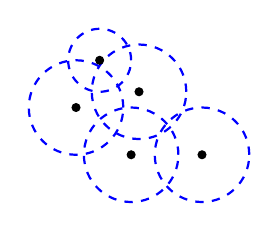
\begin{tikzpicture}
\draw[color=blue, dashed, thick](0,0) circle (0.6cm);
\draw[fill=black] (0,0) circle[radius=0.05cm];
\draw[color=blue, dashed, thick](0.8,0.2) circle (0.6cm);
\draw[fill=black] (0.8,0.2) circle[radius=0.05cm];
\draw[color=blue, dashed, thick](0.7,-0.6) circle (0.6cm);
\draw[fill=black] (0.7,-0.6) circle[radius=0.05cm];
\draw[color=blue, dashed, thick](1.6,-0.6) circle (0.6cm);
\draw[fill=black] (1.6,-0.6) circle[radius=0.05cm];
\draw[color=blue, dashed, thick](0.3,0.6) circle (0.4cm);
\draw[fill=black] (0.3,0.6) circle[radius=0.05cm];
\end{tikzpicture}
\end{figure}

Consider the open cover of $K$ given by the collection of open balls at each $p\in K$:
\[\mathcal{U}=\crbrac{B_{r_p}(p)\mid p\in E}.\]
It is clear that $\mathcal{U}$ has no finite subcover, since $E$ is infinite, and each $B_{r_p}(p)$ contains at most one point of $E$.

Since $E\subset K$, the above is also true for $K$. This contradicts the compactness of $K$.

\backward Suppose every infinite subset of $K$ that has a limit point in $K$. Fix an arbitrary open cover $\mathcal{U}=\{U_i\mid i\in I\}$ of $K$. We will show that $\mathcal{U}$ has a finite subcover, by construction.

Before that, we will reindex $\mathcal{U}$ to make it more convenient, as follows. By the definition of a cover, every $p\in K$ is contained in some $U_i$. Pick \emph{one} such $U_i$ for each $p\in K$, and call it $U_p$. Then our open cover is now $\mathcal{U}=\{U_p\mid p\in K\}$, and for all $p\in K$ we have $p\in U_p$.

\todo{To complete proof} %https://www.acsu.buffalo.edu/~achirvas/Math424_Autumn2015/cpct.pdf
\end{proof}

\begin{proposition}[Nested interval theorem]\label{prop:nested-interval}
Suppose $(I_n)$ is a decreasing sequence of closed and bounded intervals in $\RR$; that is, $I_1\supset I_2\supset\cdots$. Then
\[\bigcap_{n=1}^{\infty}I_n\neq\emptyset.\]
\end{proposition}

\begin{figure}[H]
\centering
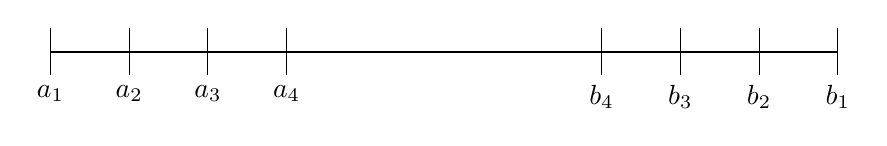
\begin{tikzpicture}
\draw[thick] (0,0) -- (10,0);
\draw (0,0.3) -- (0,-0.3) node [anchor=north] {$a_1$};
\draw (10,0.3) -- (10,-0.3) node [anchor=north] {$b_1$};
\draw (1,0.3) -- (1,-0.3) node [anchor=north] {$a_2$};
\draw (9,0.3) -- (9,-0.3) node [anchor=north] {$b_2$};
\draw (2,0.3) -- (2,-0.3) node [anchor=north] {$a_3$};
\draw (8,0.3) -- (8,-0.3) node [anchor=north] {$b_3$};
\draw (3,0.3) -- (3,-0.3) node [anchor=north] {$a_4$};
\draw (7,0.3) -- (7,-0.3) node [anchor=north] {$b_4$};
\end{tikzpicture}
\end{figure}

\begin{proof}
Let $I_n=[a_n,b_n]$, for $n=1,2,\dots$. 

Let $E=\{a_n\mid n\in\NN\}$. Since $E$ is non-empty and bounded above (by $b_1$), it has a supremum in $\RR$; let $x=\sup E$.
\begin{claim}
$\displaystyle x\in\bigcap_{n=1}^{\infty}I_n$.
\end{claim}
Since $x$ is the supremum, we have that $a_n\le x$ for all $n\in\NN$. Note that for $m>n$, $I_n\supset I_m$ implies $a_n\le a_m\le b_m\le b_n$. This means $b_n$ is an upper bound for all $a_n$; hence $x\le b_n$ for all $n\in\NN$.

Therefore $x\in I_n$ for $n=1,2,\dots$
\end{proof}

To generalise the notion of intervals, we define a \emph{$k$-cell} as
\[\{(x_1,\dots,x_k)\in\RR^k\mid a_i\le x_i\le b_i,\:1\le i\le k\}.\]

\begin{example}
A $1$-cell is an interval, a $2$-cell is a rectangle, and a $3$-cell is a rectangular solid. In this regard, we can think of a $k$-cell as a higher-dimensional version of a rectangle or rectangular solid; it is the Cartesian product of $k$ closed intervals.
\end{example}

The previous result can be generalised to $k$-cells, which we will now prove.

\begin{proposition}\label{prop:nested-interval-k-cell}
Suppose $(I_n)$ is a decreasing sequence of $k$-cells; that is, $I_1\supset I_2\supset\cdots$. Then $\bigcap_{n=1}^{\infty}I_n\neq\emptyset$.
\end{proposition}

\begin{proof}
Let $I_n$ consist of all points $\vb{x}=(x_1,\dots,x_k)$ such that
\[a_{n,i}\le x_i\le b_{n,i}\quad(1\le i\le k;\:n=1,2,\dots),\]
and put $I_{n,i}=[a_{n,i},b_{n,i}]$. For each $i$, the sequence $(I_{n,i})$ satisfies the hypotheses of \ref{prop:nested-interval}. Hence there are real numbers $x_i^\prime$ ($1\le i\le k$) such that
\[a_{n,i}\le x_i^\prime\le b_{n,i}\quad(1\le i\le k;\:n=1,2,\dots).\]
Setting $\vb{x}^\prime=(x_1^\prime,\dots,x_k^\prime)$, we see that $\vb{x}^\prime\in I_n$ for $n=1,2,\dots$. Hence $\bigcap_{n=1}^{\infty}I_n\neq\emptyset$, as desired.
\end{proof}

\begin{lemma}
Every closed interval is compact (in $\RR$).
\end{lemma}

\begin{figure}[H]
\centering
\begin{tikzpicture}
\draw[thick] (0,0) -- (10,0);
\draw (0,0.3) -- (0,-0.3) node [anchor=north] {$a$};
\draw (10,0.3) -- (10,-0.3) node [anchor=north] {$b$};
\draw (5,0.3) -- (5,-0.3) node [anchor=north] {$c_1$};
\draw (2.5,0.3) -- (2.5,-0.3) node [anchor=north] {$c_2$};
\draw (3.75,0.3) -- (3.75,-0.3) node [anchor=north] {$c_3$};
\end{tikzpicture}
\end{figure}

\begin{proof}
Suppose, for a contradiction, that a closed interval $[a,b]\subset\RR$ is not compact. Then there exists an open cover $\mathcal{U}=\{U_i\mid i\in I\}$ with no finite subcover.

Let $c_1=\frac{1}{2}(a,b)$. Subdivide $[a,b]$ into subintervals $[a,c_1]$ and $[c_1,b]$. Then $\mathcal{U}$ covers $[a,c_1]$ and $[c_1,b]$, but at least one of these subintervals has no finite subcover (if not, then both subintervals have finite subcovers, so we can take the union of the two finite subcovers to obtain a larger subcover of the entire interval). WLOG, assume $[a,c_1]$ has no finite subcover; let $I_1=[a,c_1]$.

Again subdivide $I_1$ in half to get $[a,c_2]$ and $[c_2,c_1]$. At least one of these subintervals has no finite subcover.

Repeat the above process of subdividing intervals into half. Then we obtain a decreasing sequence of closed intervals
\[I_1\supset I_2\supset I_3\supset\cdots\]
where all of them have no finite subcover of $\mathcal{U}$.

By the nested interval theorem (\ref{prop:nested-interval}), there exists $x^\prime\in I_n$ for all $n\in\NN$. Notice $x^\prime$ is in some $U_i$, which is open. Then there exists $\epsilon>0$ such that $B_\epsilon(x^\prime)\subset U_i$.

Since the length of the subintervals is decreasing and tends to zero, there exists some subinterval $I_n$ so small such that $I_n\subset B_\epsilon(x^\prime)$. This means $I_n\subset U_i$, so $U_i$ itself is an open cover of $I_n$, which contradicts the fact that $I_n$ has no finite subcover of $\mathcal{U}$.
\end{proof}

We now show a more general result.

\begin{lemma}\label{lemma:k-cell-compact}
Every $k$-cell is compact (in $\RR^k$).
\end{lemma}

\begin{proof}
We proceed in a similar manner to the proof the previous result.

Suppose $I$ is a $k$-cell; that is,
\[I=\{(x_1,\dots,x_k)\mid a_i\le x_i\le b_i,\:1\le i\le k\}.\]
Write $\vb{x}=(x_1,\dots,x_k)\in\RR^k$. Let
\[\delta=\brac{\sum_{i=1}^{k}(b_i-a_i)^2}^{1/2}\]
that is, the distance between the points $(a_1,\dots,a_k)$ and $(b_1,\dots,b_k)$, which is the maximum distance between two points in $I$: for all $\vb{x},\vb{y}\in I$,
\[|\vb{x}-\vb{y}|\le\delta.\]
Suppose, for a contradiction, that $I$ is not compact; that is, there exists an open cover $\mathcal{U}=\{U_i\}$ of $I$ which contains no finite subcover of $I$. 

For $1\le i\le k$, let $c_i=\frac{1}{2}(a_i+b_i)$. The intervals $[a_i,c_i]$ and $[c_i,b_i]$ then determine $2^k$ $k$-cells $Q_i$ whose union is $I$. At least one of these sets $Q_i$, call it $I_1$, cannot be covered by any finite subcollection of $\mathcal{U}$ (otherwise $I$ could be so covered). We next subdivide $I_1$ and continue the process. We obtain a sequence $(I_n)$ with the following properties:
\begin{enumerate}[label=(\roman*)]
\item $I\supset I_1\supset I_2\supset\cdots$
\item $I_n$ is not covered by any finite subcollection of $\mathcal{U}$
\item $|\vb{x}-\vb{y}|\le2^{-n}\delta$ for all $\vb{x},\vb{y}\in I_n$
\end{enumerate}
By (i) and \ref{prop:nested-interval-k-cell}, there is a point $\vb{x}^\prime$ which lies in every $I_n$. For some $i$, $\vb{x}^\prime\in U_i$. Since $U_i$ is open, there exists $r>0$ such that $|\vb{y}-\vb{x}^\prime|<r$ implies that $y\in U_i$. If $n$ is so large that $2^{-n}\delta<r$ (there is such an $n$, for otherwise $2^n\le\frac{\delta}{r}$ for all positive integers $n$, which is absurd since $\RR$ is archimedean), then (iii) implies that $I_n\subset U_i$, which contradicts (ii).
\end{proof}

We have now come to an important result, which will be crucial in proving the Heine--Borel theorem and Bolzano--Weierstrass theorem.

\begin{proposition}\label{prop:closed-bounded-compact-inf-lp}
If $E\subset\RR^k$ has one of the following three properties, then it has the other two:
\begin{enumerate}[label=(\roman*)]
\item $E$ is closed and bounded.
\item $E$ is compact.
\item Every infinite subset of $E$ has a limit point in $E$.
\end{enumerate}
\end{proposition}

\begin{proof} \

\fbox{(i)$\implies$(ii)} Suppose $E$ is closed and bounded. Since $E$ is bounded, then $E\subset I$ for some $k$-cell $I$.

By \ref{lemma:k-cell-compact}, $I$ is compact. Since $E$ is a closed subset of a compact set, by \ref{prop:closed-compact}, $E$ is compact.

\fbox{(ii)$\implies$(iii)} This directly follows from \ref{prop:infinite-compact-lp}.

\fbox{(iii)$\implies$(i)} If $E$ is not bounded, then $E$ contains points $\vb{x}_n$ with
\[|\vb{x}_n|>n\quad(n=1,2,3,\dots)\]
The set $S$ consisting of these points $\vb{x}_n$ is infinite and clearly has no limit point in $\RR^k$, hence has none in $E$. Thus (iii) implies that $E$ is bounded.

If $E$ is not closed, then there is a point $\vb{x}_0\in\RR^k$ which is a limit point of $E$ but not a point of $E$. For $n=1,2,3,\dots$, there are points $\vb{x}_n\in E$ such that $|\vb{x}_n-\vb{x}_0|<\frac{1}{n}$. Let $S$ be the set of these points $\vb{x}_n$. Then $S$ is infinite (otherwise $|\vb{x}_n-\vb{x}_0|$ would have a constant positive value, for infinitely many $n$), $S$ has $\vb{x}_0$ as a limit point, and $S$ has no other limit point in $\RR^k$. For if $\vb{y}\in\RR^k$, $\vb{y}\neq\vb{x}_0$, then
\begin{align*}
|\vb{x}_n-\vb{y}|&\ge|\vb{x}_0-\vb{y}|-|\vb{x}_n-\vb{x}_0|\\
&\ge|\vb{x}_0-\vb{y}|-\frac{1}{n}\\
&\ge\frac{1}{2}|\vb{x}_0-\vb{y}|
\end{align*}
for all but finitely many $n$; this shows that $\vb{y}$ is not a limit point of $S$ (Theorem 2.20).

Thus $S$ has no limit point in $E$; hence $E$ must be closed if (iii) holds.\todo{review proof}
\end{proof}

\begin{theorem}[Heine--Borel theorem]\label{thrm:heine-borel}
$E\subset\RR^n$ is compact if and only if $E$ is closed and bounded.
\end{theorem}

\begin{proof}
This is simply (i)$\iff$(ii) in the previous result.
\end{proof}

\subsection{Bolzano--Weierstrass Theorem}
\begin{theorem}[Bolzano--Weierstrass theorem]\label{thrm:bolzano-weierstrass}
Every bounded infinite subset of $\RR^n$ has a limit point in $\RR^n$.
\end{theorem}

\begin{proof}
Suppose $E$ is a bounded infinite subset of $\RR^n$.

Since $E$ is bounded, there exists an $n$-cell $I\subset\RR^n$ such that $E\subset I$. Since $I$ is compact, by \ref{prop:infinite-compact-lp}, $E$ has a limit point in $I$ and thus $\RR^n$. 
\end{proof}
\pagebreak

\subsection{Cantor's Intersection Theorem}
A collection $\mathcal{A}$ of subsets of $X$ is said to have the \emph{finite intersection property} if the intersection of every finite subcollection of $\mathcal{A}$ is non-empty.

\begin{proposition}\label{prop:finite-intersection-property}
Suppose $\mathcal{K}=\{K_i\mid i\in I\}$ is a collection of compact subsets of a metric space $X$, which satisfies the finite intersection property. Then $\bigcap_{i\in I}K_i\neq\emptyset$.
\end{proposition}

\begin{proof}
We fix a member $K_1\subset\mathcal{K}$. Suppose, for a contradiction, that $\bigcap_{i\in I}K_i=\emptyset$; that is, no point of $K_1$ belongs to every $K_i\in\mathcal{K}$. 

For $i\in I$, let $U_i={K_i}^c$. Then the sets $\{U_i\mid i\in I\}$ form an open cover of $K_1$. Since $K_1$ is compact by assumption, there exist finitely many indices $i_1,\dots,i_n$ such that
\[K_1\subset\bigcup_{k=1}^{n}U_{i_k}.\]
By de Morgan's laws, we have that
\[\bigcup_{k=1}^{n}U_{i_k}=\bigcup_{k=1}^{n}{K_{i_k}}^c=\brac{\bigcap_{k=1}^{n}K_{i_k}}^c.\]
Thus
\[K_1\subset\brac{\bigcap_{k=1}^{n}K_{i_k}}^c,\]
which means that
\[K_1\cap\bigcap_{k=1}^{n}K_{i_k}=\emptyset.\]
Thus $K_1,K_{i_1},\dots,K_{i_n}$ is a finite subcollection of $\mathcal{K}$ which has an empty intersection; this contradicts the finite intersection property of $\mathcal{K}$.
\end{proof}

\begin{theorem}[Cantor's intersection theorem]\label{thrm:cantor-intersection}
Suppose $(K_n)$ is a decreasing sequence of non-empty compact sets; that is, $K_1\supset K_2\supset\cdots$. Then $\bigcap_{n=1}^\infty K_n\neq\emptyset$.
\end{theorem}

\begin{proof}
This is an immediate corollary of the previous result.
\end{proof}

The following result is a characterisation of compact sets.

\begin{proposition}
$K$ is compact if and only if every collection of closed subsets of $K$ satisfies the finite intersection property.
\end{proposition}

\begin{proof} \

\forward Suppose $K$ is compact.

If $\mathcal{U}$ is an open covering of $K$, then the collection $\mathcal{F}$ of complements of sets in $\mathcal{U}$ is a collection of closed sets whose intersection is empty (why?); and 

conversely, if $\mathcal{F}$ is a collection of closed sets whose intersection is empty, then the collection $\mathcal{U}$ of complements of sets in $\mathcal{F}$ is an open covering.

\todo{To complete proof} %https://www.ucl.ac.uk/~ucahad0/3103_handout_2.pdf
\end{proof}
\pagebreak

\subsection{Sequential Compactness}
\begin{definition}[Sequential compactness]
We say $K\subset X$ is \vocab{sequentially compact} if every sequence in $K$ has a convergent subsequence in $K$.
\end{definition}

We now show that compactness and sequential compactness are equivalent.

\begin{proposition}
$K\subset X$ is compact if and only if it is sequentially compact.
\end{proposition}

\begin{proof} \

\forward Suppose $K\subset X$ is compact. Take any sequence $(y_n)$ from $K$. Suppose, for a contradiction, that every point $x\in K$ is not a limit of any subsequence of $(y_n)$. Then for all $x\in K$, there exists $r_x>0$ such that $B_{r_x}(x)$ contains at most one point in $(y_n)$, which is $x$.

Consider the collection of open balls at each $x\in K$:
\[\{B_{r_x}(x)\mid x\in K\}.\]
This is an open cover of $K$. By the compactness of $K$, there exists a finite subcover of $K$:
\[\crbrac{B_{r_{x_1}}(x_1),\dots,B_{r_{x_N}}(x_N)}.\]
In particular, these open balls cover $\{y_n\}$. Hence there must be some $x_i$ ($1\le i\le N$) such that there are infinitely many $y_j=x_i$. Consider the sequence $(y_j)$ where each term in this sequence is equal to $x_i$; this is a subsequence of $(y_n)$ that converges to $x_i\in K$. This contradicts the assumption.

\backward Suppose, for a contradiction, that $K$ is not compact. Then there exists an open cover $\{U_\alpha\mid \alpha\in \Lambda_\alpha\}$ which has no finite subcover. Then $\Lambda$ must be an infinite set.

If $\Lambda$ is countable, WLOG, assume $\Lambda=\NN$. Since any finite union
\[\bigcup_{i=1}^{n}U_i\]
cannot cover $K$, we can take some $x_n\in K\setminus\bigcup_{i=1}^{n}U_i$ for every $n\in\NN$. Then we obtain a sequence $(x_n)$ in $K$ and so must have a convergent subsequence $(x_{n_k})$ that converges to some $x_0\in K$. It follows that there must be some $U_N$ such that $x_0\in U_N$. Since $U_N$ is open, there exists $r>0$ such that 
\[B_r(x_0)\subset U_N.\]
On the other hand, since $x_{n_k}\to x_0$, there exists $N^\prime\in\NN$ such that if $n_k\ge N^\prime$ then
\[x_{n_k}\in B_r(x_0).\]
However, by our way of choosing $x_n$, whenever $n_k>\max\{N^\prime,N\}$, $x_{n_k}\notin U_N$. This leads to a contradiction.
\end{proof}
\pagebreak

\section{Perfect Sets}
\subsection{Definition and Uncountability}
\begin{definition}[Perfect set]
$E$ is \vocab{perfect}\index{perfect set} if
\begin{enumerate}[label=(\roman*)]
\item $E$ is closed, and
\item every point of $E$ is a limit point of $E$.
\end{enumerate}
\end{definition}

\begin{proposition}
Let non-empty $P\subset\RR^k$ be perfect. Then $P$ is uncountable.
\end{proposition}

\begin{proof}
Since $P$ has limit points, by \ref{prop:limit-point-inf-points}, $P$ is an infinite set.

Suppose, for a contradiction, that $P$ is countable. This means we can list the points of $P$ in a sequence:
\[\vb{x}_1,\vb{x}_2,\vb{x}_3,\dots\]
Consider a sequence $(B_n)$ of open balls, where $B_n$ is any open ball centred at $\vb{x}_n$:
\[B_n=\crbrac{\vb{y}\in\RR^k\:\big|\:|\vb{y}-\vb{x}_n|<r}.\]
Then its closure $\overline{B_n}$ is the closed ball
\[\overline{B}_n=\crbrac{\vb{y}\in\RR^k\:\big|\:|\vb{y}-\vb{x}_n|\le r}.\]
Suppose $B_n$ has been constructed. Note that $B_n\cap P$ is not empty. Since $P$ is perfect, every point of $P$ is a limit point of $P$, so there exists $B_{n+1}$ such that (i) $\overline{B}_{n+1}\subset B_n$, (ii) $\vb{x}_n\notin\overline{B}_{n+1}$, (iii) $B_{n+1}\cap P$ is not empty. 

By (iii), $B_{n+1}$ satisfies our induction hypothesis, and the construction can proceed. 

Put $K_n=\overline{B}_n\cap P$. Since $\overline{B}_n$ is closed and bounded, $\overline{B}_n$ is compact. Since $\vb{x}_n\notin K_{n+1}$, no point of $P$ lies in $\bigcap_{n=1}^{\infty}K_n$. Since $K_n\subset P$, this implies that $\bigcap_{n=1}^{\infty}K_n$ is empty. But each $K_n$ is nonempty, by (iii), and $K_n\supset K_{n+1}$ by (i); this contradicts Cantor's intersection theorem (\ref{thrm:cantor-intersection}).
\end{proof}

\begin{corollary*}
Every interval $[a,b]$ is uncountable. In particular, $\RR$ is uncountable.
\end{corollary*}
\pagebreak

\subsection{Cantor Set}
We now construct the Cantor set. Consider the interval
\[C_0=[0,1].\]
Remove the middle third $\brac{\frac{1}{3},\frac{2}{3}}$ to give
\[C_1=\sqbrac{0,\frac{1}{3}}\cup\sqbrac{\frac{2}{3},1}.\]
Remove the middle thirds of these intervals to give
\[C_2=\sqbrac{0,\frac{1}{9}}\cup\sqbrac{\frac{2}{9},\frac{3}{9}}\cup\sqbrac{\frac{6}{9},\frac{7}{9}}\cup\sqbrac{\frac{8}{9},1}.\]

\begin{figure}[H]
\centering
\begin{tikzpicture}
\draw (9,0) -- (0,0) node [anchor=east] {$C_0$};
\draw (9,-1) -- (6,-1);
\draw (3,-1) -- (0,-1) node [anchor=east] {$C_1$};
\draw (9,-2) -- (8,-2);
\draw (7,-2) -- (6,-2);
\draw (3,-2) -- (2,-2);
\draw (1,-2) -- (0,-2) node [anchor=east] {$C_2$};
\end{tikzpicture}
\caption{Cantor set}
\end{figure}

Repeating this process, we obtain a monotonically decreasing sequence of compact sets $(C_n)$, where $C_n$ is the union of $2^n$ intervals, each of length $3^{-n}$. Recursively, we have that $C_{n+1}=\frac{1}{3}C_n\cup\brac{\frac{1}{3}C_n+\frac{2}{3}}$.

Note that each $C_n$ has the following properties:
\begin{enumerate}[label=(\roman*)]
\item closed (since each $C_n$ is a finite union of closed sets, which is closed)
\item compact (since each $C_n$ is a closed subset of a compact set $[a,b]$)
\item non-empty (since the endpoints $0$ and $1$ are in each $C_n$)
\end{enumerate}

The \vocab{Cantor set} is defined to be the union
\[C\colonequals\bigcap_{n=1}^{\infty}C_n.\]

\begin{lemma}[Properties of the Cantor set] \
\begin{enumerate}[label=(\roman*)]
\item $C$ is closed.
\item $C$ is compact.
\item $C$ is not empty.
\item $C$ has no interior points.
\end{enumerate}
\end{lemma}

\begin{proof} \
\begin{enumerate}[label=(\roman*)]
\item $C$ is the intersection of arbitrarily many closed sets, so $C$ is closed.
\item $C$ is bounded in $[0,1]$, by definition. Since $C$ is closed and bounded, by the Heine--Borel theorem, $C$ is compact.
\item Since $(C_n)$ is a decreasing sequence of non-empty compact sets, by Cantor's intersection theorem, $\bigcap_{n=1}^{\infty}C_n=C\neq\emptyset$.
\item Suppose, for a contradiction, that there exists $p\in C$ which is an interior point. Then there exists some open interval around $p$, i.e., $p\in(a,b)$.

However in $C_n$, each interval has length $\frac{1}{3^n}$. Hence for any $(a,b)$ we can find some $n\in\NN$ such that $(a,b)$ is not contained in $C_n$ and hence not contained in $C$.
\end{enumerate}
\end{proof}

\begin{proposition}
$C$ is a perfect set in $\RR$ which contains no open interval.
\end{proposition}

\begin{proof}
We will show that (i) $C$ contains no open interval, and (ii) $C$ is perfect.
\begin{enumerate}[label=(\roman*)]
\item No open interval of the form
\[\brac{\frac{3k+1}{3^m},\frac{3k+2}{3^m}},\]
where $k,m\in\ZZ^+$, has a point in common with $C$. Since every open interval $(\alpha,\beta)$ contains a open interval of the above form, if
\[3^{-m}<\frac{\beta-\alpha}{6},\]
$C$ contains no open interval.

\item Sincw we have shown that $C$ is closed, it suffices to show that every point of $C$ is a limit point.

Let $x\in C$, and let $S$ be any open interval containing $x$. Let $I_n$ be that interval of $C_n$ which contains $x$. Choose $n$ large enough, so that $I_n\subset S$. Let $x_n$ be an endpoint of $I_n$, such that $x_n\neq x$.

It follows from the construction of $C$ that $x_n\in P$. Hence $x$ is a limit point of $C$, and $C$ is perfect.
\end{enumerate}
\end{proof}

\begin{corollary}
$C$ is uncountable.
\end{corollary}

One of the most interesting properties of the Cantor set is that it provides us with an example of an uncountable set of measure zero.
\pagebreak

\section{Connectedness}
\begin{definition}[Connectedness]
We say $A$ and $B$ are \vocab{separated} if
\begin{enumerate}[label=(\roman*)]
\item $A\cap\overline{B}=\emptyset$, and
\item $\overline{A}\cap B=\emptyset$;
\end{enumerate}
that is, no point of $A$ lies in the closure of $B$, and no point of $B$ lies in the closure of $A$. (Equivalently, no point of one set is a limit point of the other set.)

$E\subset X$ is \vocab{connected}\index{connectedness} if $E$ is not the union of two non-empty separated sets. 
\end{definition}

\begin{remark}
Separated sets are of course disjoint, but disjoint sets need not be separated. For example, $[0,1]$ and $(1,2)$ are not separated, since $1$ is a limit point of $(1,2)$. However $(0,1)$ and $(1,2)$ are separated.
\end{remark}

\begin{example}
In $\RR^2$, consider the set
\[E=\{(x,y)\mid x,y\in\QQ\}.\]
Then $E$ is not connected; if we let
\begin{align*}
A&=\crbrac{(x,y)\mid x,y\in\QQ,x<\sqrt{2}},\\
B&=\crbrac{(x,y)\mid x,y\in\QQ,x>\sqrt{2}},
\end{align*}
then note that $A\cup B=E$, as well as $A\cap\overline{B}=\emptyset$ and $\overline{A}\cap B=\emptyset$.
\end{example}

\begin{lemma}\label{lemma:connected-closed-interval}
Closed intervals in $\RR$ are connected.
\end{lemma}

\begin{proof}
Suppose, for a contradiction, that a closed interval $[a,b]$ is not connected. Then there exists non-empty sets $A$ and $B$, with $A\cap\overline{B}=\emptyset$ and $\overline{A}\cap B=\emptyset$. WLOG let $a\in A$.

Let $s=\sup A$. By \ref{lemma:closure-sup}, $s\in\overline{A}$. Then $\overline{A}\cap B=\emptyset$ implies $s\notin B$, so $s\in A$. Thus $A\cap\overline{B}=\emptyset$ implies $s\notin\overline{B}$. Hence there exists an open interval $(s-\epsilon,s+\epsilon)$ around $s$ that is disjoint from $B$. But since $A\cup B=[a,b]$, we must have $(s-\epsilon,s+\epsilon)\subset A$. This contradicts the fact that $s$ is the supremum of $A$. 
\end{proof}

The connected subsets of the real line have a particularly simple structure: 

\begin{lemma}\label{lemma:connected-interval-R}
$E\subset\RR$ is connected if and only if it has the following property: if $x,y\in E$ and $x<z<y$, then $z\in E$.
\end{lemma}

\begin{proof} \

\backward If there exists $x,y\in E$ and some $z\in(x,y)$ such that $z\notin E$, then $E=A_z\cup B_z$ where
\[ A_z=E\cap(-\infty,z), \quad B_z=E\cap(z,\infty). \]
Since $x\in A_z$ and $y\in B_z$, $A$ and $B$ are non-empty. Since $A_z\subset(-\infty,z)$ and $B_z\subset(z,\infty)$, they are separated. Hence $E$ is not connected.

\forward Suppose $E$ is not connected. Then there are non-empty separated sets $A$ and $B$ such that $A\cup B=E$. Pick $x\in A$, $y\in B$, and WLOG assume that $x<y$. Define
\[z\colonequals\sup(A\cap[x,y].)\]
By \ref{lemma:closure-sup}, $z\in\overline{A}$; hence $z\notin B$. In particular, $x\le z<y$.
\begin{description}
\item[Case 1: $z\notin A$.] It follows that $x<z<y$ and $z\notin E$.
\item[Case 2: $z\in A$.] Then $z\notin B$, hence there exists $z_1$ such that $z<z_1<y$ and $z_1\notin B$. Then $x<z_1<y$ and $z_1\notin E$.
\end{description}
\end{proof}
\pagebreak

\subsection{Path Connectedness}

\pagebreak

\section{Separable Spaces}
\begin{definition}[Separable space]
$X$ is \vocab{separable} if it has a countable subset which is dense in $X$.
\end{definition}

\begin{example} \
\begin{itemize}
\item $\RR$ is separable.
\begin{proof}
The set of rational numbers $\QQ$ is countable and is dense in $\RR$.
\end{proof}

\item $\CC$ is separable.
\begin{proof}
A countable dense subset of $\CC$ is the set of all complex numbers whose real and imaginary parts are both rational, i.e., the set $\{x+yi\mid x,y\in\QQ\}$.
\end{proof}

\item The \emph{discrete metric space} $X$ is separable if and only if $X$ is countable.
\begin{proof}
The kind of metric implies that no proper subset of $X$ can be dense in $X$. Hence the only dense set in $X$ is $X$ itself, and the statement follows. 
\end{proof}

\item The \emph{sequence space} $\ell^\infty$ is the set of all bounded complex sequences, with the metric defined by
\[d(x,y)=\sup_{n\in\NN}|x_n-y_n|.\]
$\ell^\infty$ is not separable.
\end{itemize}
\end{example}
\pagebreak

\section{Baire Category Theorem}
%https://www.ucl.ac.uk/~ucahad0/3103_handout_7.pdf
$E\subset X$ is called \vocab{nowhere dense} (in $X$) if the interior of the closure of A is empty, i.e., $(\overline{A})^\circ=\emptyset$. 

Otherwise put, $E$ is nowhere dense iff it is contained in a closed set with empty interior. Passing to complements, we can say equivalently that $E$ is nowhere dense iff its complement contains a dense open set (why?).

\begin{lemma}
Let $X$ be a metric space.
\begin{enumerate}[label=(\roman*)]
\item Any subset of a nowhere dense set is nowhere dense.
\item The union of finitely many nowhere dense sets is nowhere dense.
\item The closure of a nowhere dense set is nowhere dense.
\item If $X$ has no isolated points, then every finite set is nowhere dense.
\end{enumerate}
\end{lemma}

\begin{proof} \
\begin{enumerate}[label=(\roman*)]
\item 
\item 
\item 
\item 
\end{enumerate}
\end{proof}

Although the union of finitely many nowhere dense sets is nowhere dense, the union of countably many nowhere dense sets need not be nowhere dense: for instance, in $X=\RR$, the rationals $\QQ$ are the union of countably many nowhere dense sets (why?), but the rationals are certainly not nowhere dense (indeed, they are everywhere dense, i.e. $(\overline{\QQ})^\circ=\overline{\QQ}=\RR$).

This observation motivates the introduction of a larger class of sets: $A\subset X$ is called \vocab{meager} (or of first category) in $X$ if it can be written as a countable union of nowhere dense sets; otherwise, it is \emph{non-meager} (or of second category). The complement of a meager set is called \vocab{residual}.

We then have as an immediate consequence:

\begin{lemma}
Let $X$ be a metric space.
\begin{enumerate}[label=(\roman*)]
\item Any subset of a meager set is meager.
\item The union of countably many meager sets is meager.
\item If $X$ has no isolated points, then every countable set is meager.
\end{enumerate}
\end{lemma}

We are now ready to state the Baire category theorem.

\begin{theorem}[Baire category theorem]
Let $X$ be a complete metric space.
\begin{enumerate}[label=(\roman*)]
\item A meager set has empty interior.
\item The complement of a meager set is dense. (That is, a residual set is dense.)
\item A countable intersection of dense open sets is dense.
\end{enumerate}
\end{theorem}

You should carefully verify that (i), (ii) and (iii) are equivalent statements, obtained by taking complements.

In applications we frequently need only the weak form of the Baire category theorem that is obtained by weakening ``is dense'' in (b,c) to ``is non-empty'' (which is valid whenever $X$ is itself non-empty):

\begin{corollary}[Weak form of the Baire category theorem]
Let $X$ be a non-empty complete metric space.
\begin{enumerate}[label=(\roman*)]
\item $X$ cannot be written as a countable union of nowhere dense sets. (In other words, $X$ is nonmeager in itself.)
\item If $X$ is written as a countable union of closed sets, then at least one of those closed sets has nonempty interior.
\item A countable intersection of dense open sets is nonempty.
\end{enumerate}
\end{corollary}

\pagebreak

\section*{Exercises}
\begin{exercise}
Prove that the following are metrics.
\begin{enumerate}[label=(\roman*)]
\item On an arbitrary set $X$, define
\[d(x,y)=\begin{cases}
1&(x\neq y)\\
0&(x=y)
\end{cases}\]
(This is called the \emph{discrete metric}.)

\item On $\ZZ$, define $d(x,y)$ to be $2^{-m}$, where $2^m$ is the largest power of two dividing $x-y$. The triangle inequality holds in the following stronger form, known as the ultrametric property:
\[d(x,z)\le\max\{d(x,y),d(y,z)\}.\]
Indeed, this is just a rephrasing of the statement that if $2^m$ divides both $x-y$ and $y-z$, then $2^m$ divides $x-z$.

(This is called the \emph{2-adic metric}. The role of $2$ can be replaced by any other prime $p$, and the metric may also be extended in a natural way to the rationals $\QQ$.)

\item Let $\mathcal{G}=(V,E)$ be a connected graph. Define $d$ on $V$ as follows: $d(v,v)=0$, and $d(v,w)$ is the length of the shortest path from $v$ to $w$.

(This is known as the \emph{path metric}.)

\item Let $G$ be a group generated by elements $a$, $b$ and their inverses. Define a distance on $G$ as follows: $d(v,w)$ is the minimal $k$ such that $v=wg_1\cdots g_k$, where $g_i\in\{a,b,a^{-1},b^{-1}\}$ for all $i$.

(This is known as the \emph{word metric}.)

\item Let $X=\{0,1\}^n$ (the boolean cube), the set of all strings of $n$ zeroes and ones. Define $d(x,y)$ to be the number of coordinates in which $x$ and $y$ differ.

(This is known as the \emph{Hamming distance}.)

\item Consider the set $P(\RR^n)$ of one-dimensional subspaces of $\RR^n$, that is to say lines through the origin. One way to define a distance on this set is to take, for lines $L_1,L_2$, the distance between $L_1$ and $L_2$ to be
\[d(L_1,L_2)=\sqrt{1-\frac{|\langle v,w\rangle|^2}{\norm{v}^2\norm{w}^2}},\]
where $v$ and $w$ are any non-zero vectors in $L_1$ and $L_2$ respectively.

When $n=2$, the distance between two lines is $\sin\theta$ where $\theta$ is the angle between those lines.

(This is known as the \emph{projective space}.)
\end{enumerate}
\end{exercise}

\begin{exercise}[Product space]
If $(X,d_X)$ and $(Y,d_Y)$ are metric spaces, set
\[d_{X\times Y}\brac{(x_1,y_1),(x_2,y_2)}=\sqrt{d_X(x_1,x_2)^2+d_Y(y_1,y_2)^2.}\]
for $x_1,x_2\in X$, $y_1,y_2\in Y$.

Prove that $d_{X\times Y}$ gives a metric on $X\times Y$; we call $X\times Y$ the \emph{product space}.
\end{exercise}

\begin{solution}
Reflexivity and symmetry are obvious. Less clear is the triangle inequality. We need to prove that
\begin{equation*}\tag{1}
\begin{split}
&\sqrt{d_X(x_1,x_3)^2+d_Y(y_1,y_3)^2}+\sqrt{d_X(x_3,x_2)^2+d_Y(y_3,y_2)^2}\\
&\ge\sqrt{d_X(x_1,x_2)^2+d_Y(y_1,y_2)^2}
\end{split}
\end{equation*}
Write $a_1=d_X(x_2,x_3)$, $a_2=d_X(x_1,x_3)$, $a_3=d_X(x_1,x_2)$ and similarly $b_1=d_Y(y_2,y_3)$, $b_2=d_Y(y_1,y_3)$ and $b_3=d_Y(y_1,y_2)$. Thus we want to show
\begin{equation*}\tag{2}
\sqrt{{a_2}^2+{b_2}^2}+\sqrt{{a_1}^2+{b_1}^2}\ge\sqrt{{a_3}^2+{b_3}^2}.
\end{equation*}
To prove this, note that from the triangle inequality we have $a_1+a_2\ge a_3$, $b_1+b_2\ge b_3$. Squaring and adding gives
\[{a_1}^2+{b_1}^2+{a_2}^2+{b_2}^2+2(a_1a_2+b_1b_2)\ge {a_3}^2+{b_3}^2.\]
By Cauchy--Schwarz,
\[a_1a_2+b_1b_2\le\sqrt{{a_1}^2+{b_1}^2}\sqrt{{a_2}^2+{b_2}^2}.\]
Substituting this into the previous line gives precisely the square of (2), and (1) follows.
\end{solution}

